\chapter*{neurodivergent}
\addcontentsline{toc}{chapter}{neurodivergent}
\begin{center}
\vspace{2cm}
\begin{flushright}
\large
\textit{The holographic principle suggests that information about a volume of space can be encoded on its boundary, leading to a perspective in which spacetime within that volume, including time, is a projection. Thus, time might not exist as a fundamental property but instead as a result of interactions in this deeper, more fundamental layer of reality.}
\end{flushright}
\vspace{2cm}
\end{center}
\normalsize

\newpage 
The idea of perception as a controlled hallucination suggests that what we see, know, and understand is no more than the most likely prediction made by our trained brains. A neural network in which an internal conflict arises between an error signal, indicating that what's in front of us does not match our expectations, and a massively skewed training dataset of memories, insisting that what we know from past experiences is the correct interpretation.

Neurodivergence is now better known and understood, but as a statistical minority, it is not well represented in the dataset of human interactions. It is only logical that it would be difficult to comprehend from the perspective of a neurotypical brain. The issue of skewed datasets is commonly addressed in the context of AI and machine learning. However, while we can design datasets to balance the represented populations, a real brain learns from real interactions, and the statistics remain the same regardless of awareness.

\textit{"Anything in the territory that resists attempts at modeling thus becomes, in the world of digital models, noise in the system"} \citep{benasayag2019}. Benasayag addresses the issue of algorithmic bias, where neural networks may perpetuate existing social prejudices and inequalities. He underscores the need for critical examination of the data and methodologies used in AI to prevent reinforcing discriminatory practices.

Benasayag's insight raises concerns about the way AI and algorithmic models structure knowledge, representation, and power. This encourages a critical interrogation of locality, which, in digital and algorithmic contexts, is often flattened, abstracted, or omitted in favor of more "universal" models. Problematizing locality involves examining how algorithmic systems fail to account for the specificity of place, culture, history, and identity, reinforcing biases embedded in generalized datasets.

The holographic principle challenges the classical idea of locality, suggesting that information can have non-local representations. As a neurodivergent individual, cause-and-effect thinking strategies don't come naturally, favoring lateral connections and holistic insights that reflect non-locality in thought processes. Often a heightened awareness of details, turns into an intuitive grasp of the whole system encoded in parts, as a kind of cognitive holography. Most attempts to uncompress this intuition often come across as confusing misunderstandings, since even language is made to reflect linear interpretations of reality through sequential narratives.

{\scriptsize \textcolor{comment}{\% Exist within the noise }}

RANSAC (RANdom SAmple Consensus) is an iterative algorithm used for estimating the parameters of a mathematical model from a dataset that contains both inliers (data points that fit the model) and outliers (data points that do not fit the model). See Figure~\ref{fig:ransac}. It is particularly robust and capable of rejecting outliers and is widely used in applications in the presence of noise. We must define new non-probabilistic approaches to social norms and rules that includes outliers, or avoid the models and rules altogether, validating the richness of the full spectrum, avoiding the expectations of coherence to the known set. 

%% image
\begin{figure}
    \centering
    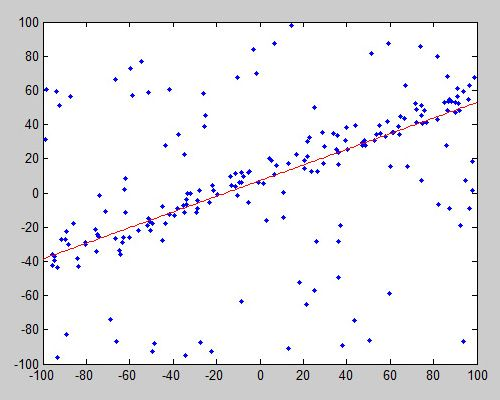
\includegraphics[width=0.8\linewidth]{assets/ransac.jpg} 
    \caption{\small Data points shown in blue, with the line of form y = mx+c estimated using RANSAC indicated in red. - \textit{https://www.mathworks.com}.}
    \label{fig:ransac}
\end{figure}

Algorithms for pattern recognition, collapse heterogeneous realities into standardized, data-driven abstractions. However, certain local specificities do not easily conform to the logic of machine learning. These \textit{"outliers"} or \textit{"anomalies"} are often treated as statistical noise, rather than meaningful divergences that could challenge the system's assumptions. Problematizing locality, then, requires acknowledging that what is excluded from modeling is not neutral but politically significant.

AI models often depend on data extracted from local contexts but are deployed in a non-localized, decontextualized manner. This reinforces structural inequalities, where data from marginalized communities is used to optimize systems that do not serve them, or actively oppress them (e.g., urban surveillance and predictive policing).

{\scriptsize \textcolor{comment}{\% Analytical acceptance, algorithmic forgiveness. }}

I went through many struggles conforming to neurotypical norms. As a child, I used to write mirrored text and had difficulty reading, so I was quickly diagnosed with dyslexia. I suffered from insomnia for a big portion of my adolescence, as a result of the discomforts of forced social interactions. Later in life, I was prescribed with medication for anxiety disorders due to unbearable panic attack seasons. I was diagnosed quite late in life with ADHD (Attention Deficit Hyperactivity Disorder), followed with a possible co-occurrence of ASD (Autism Spectrum Disorder), a mixed condition that affects a small percentage of the population\footnote{ADHD has a global prevalence of around 5-7\% of children and 2-5\% of adults. Around 20-50\% of individuals with ADHD also meet criteria for ASD.}. I started making sense of the previous 40 years, the anxiety, the insomnia, the lack of personal memories, and the depression caused by simply not fitting-in. I came to realize that a deeper knowledge and understanding of this region of the spectrum became my way of making sense of my interactions with the world, allowing me to forgive myself and others, while also developing the necessary rational arguments to actively reject the structures responsible for perpetuating the generalized norms that shape our societies.

{\scriptsize \textcolor{comment}{\% symbiotic contamination}}

In the current context of a neurotypical majority, forging the options and leading to a society that values selection over creativity, the creation of our own tools seems to be an appropriate choice to true creativity. Such practices allow to dig into deeper understanding of the final outcomes, and explore the equally rich properties of every step of a process.  

\subsection*{time scales}

For some neurodivergent individuals, time feels less sequential and more layered or interconnected, as if different dimensions of experience coexist and interact simultaneously. Moments may feel fragmented, time may be experienced in hyperfocus (expanding infinitely) or in rapid, disjointed flashes. Much like a hologram contains a vast amount of information compressed into a simpler lower-dimensional form, neurodivergent cognition could compress complex timelines and experiences into non-linear formats, creating unique interpretations and associations across time.
Neurodivergent cognition might operate by projecting internal mental states or processing vast amounts of sensory data into condensed forms like patterns, metaphors, or unique associations. 

Deleuze's concept of the \textit{"irrational cut"} in cinema\footnote{Deleuze frequently references Godard as a master of the "irrational cut"}, introduced in "\textit{Cinema 2: The Time-Image}"\citep{deleuze1985}, marks a fundamental disruption of classical continuity and logical progression in film editing. Unlike the \textit{"rational cut"} of classical cinema, which follows a clear cause-and-effect chain, the irrational cut severs this logical flow, creating temporal and spatial disjunctions that do not adhere to conventional narrative logic. Instead, these cuts generate pure time-images, where past, present, and future may coexist in ambiguous and nonlinear ways.

This disruption of linearity in cinema resonates deeply with neurodivergent modes of perception and cognition, particularly in conditions such as ADHD, autism, and certain forms of synesthesia, where experiences of time, memory, and causality often do not conform to neurotypical expectations.

Many neurodivergent individuals experience thought processes that operate in a non-hierarchical, associative, or rhizomatic manner. Rather than following a clear sequence, thoughts, memories, and perceptions may form intricate networks where disparate elements become linked without a clear rational justification. This mirrors how the irrational cut allows film sequences to be connected not through logic, but through affect, intuition, or symbolic resonance.
 
{\scriptsize \textcolor{comment}{\% failures with a serial number}}

I'm interested in multi-sensory installations, layered audio-visual compositions, or interactive works that allow viewers to experience various \textit{"time slices"} of the piece, where events and emotions compress into a single moment. Experiences of layered and non-linear time are certainly an inspiration to an approach that defies linear storytelling or straightforward interaction.

{\scriptsize \textcolor{comment}{\% examples}}

In his Theater Series, Figure~\ref{fig:sugimoto}, Hiroshi Sugimoto \citep{sugimotohiroshi} created a series of long-exposure photographs of cinemas where an entire film is projected onto a single frame, collapsing a full-length movie into a single luminous image. Similarly, in Figure~\ref{fig:mv01}, a digital work of my own authorship, the equation for incremental mean calculation is implemented to run over video sequences, presenting time not as linear but as an accumulation of all its moments at once.

The generative installation titled \textit{"33 Questions per Minute"}, by Rafael Lozano-Hemmer \citep{lozano-hemmer}, Figure~\ref{fig:lozano}, shows a rapidly changing sequence of randomly generated questions on LCD screens, exceeding the speed at which they can be read. This creates a layered simultaneity of potential meanings and missed moments in time.

%% image
\begin{figure}
    \centering
    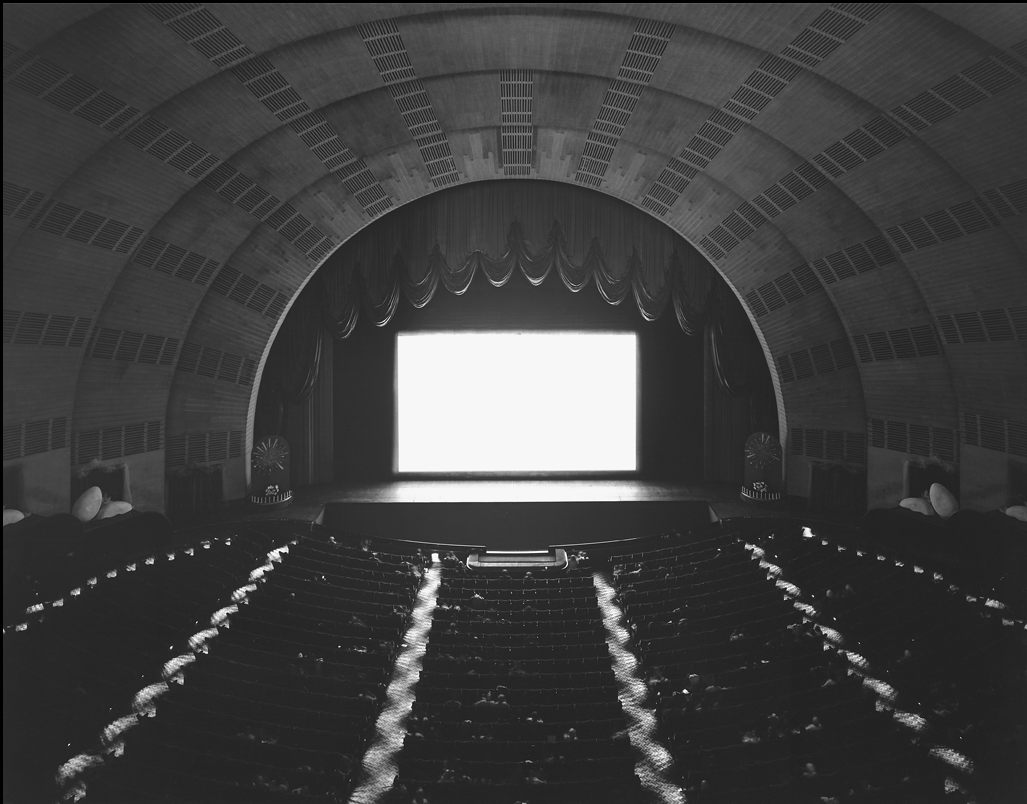
\includegraphics[width=0.8\linewidth]{assets/hiroshi-sugimoto-theaters-1978-1993-Radio-City-Music-Hall-1.png} 
    \caption{\small  Radio City Music Hall, New York 1978 - \textit{Hiroshi Sugimoto, Theaters, https://yoshiigallery.com}.}
    \label{fig:sugimoto}
\end{figure}


%% image
\begin{figure}
    \centering
    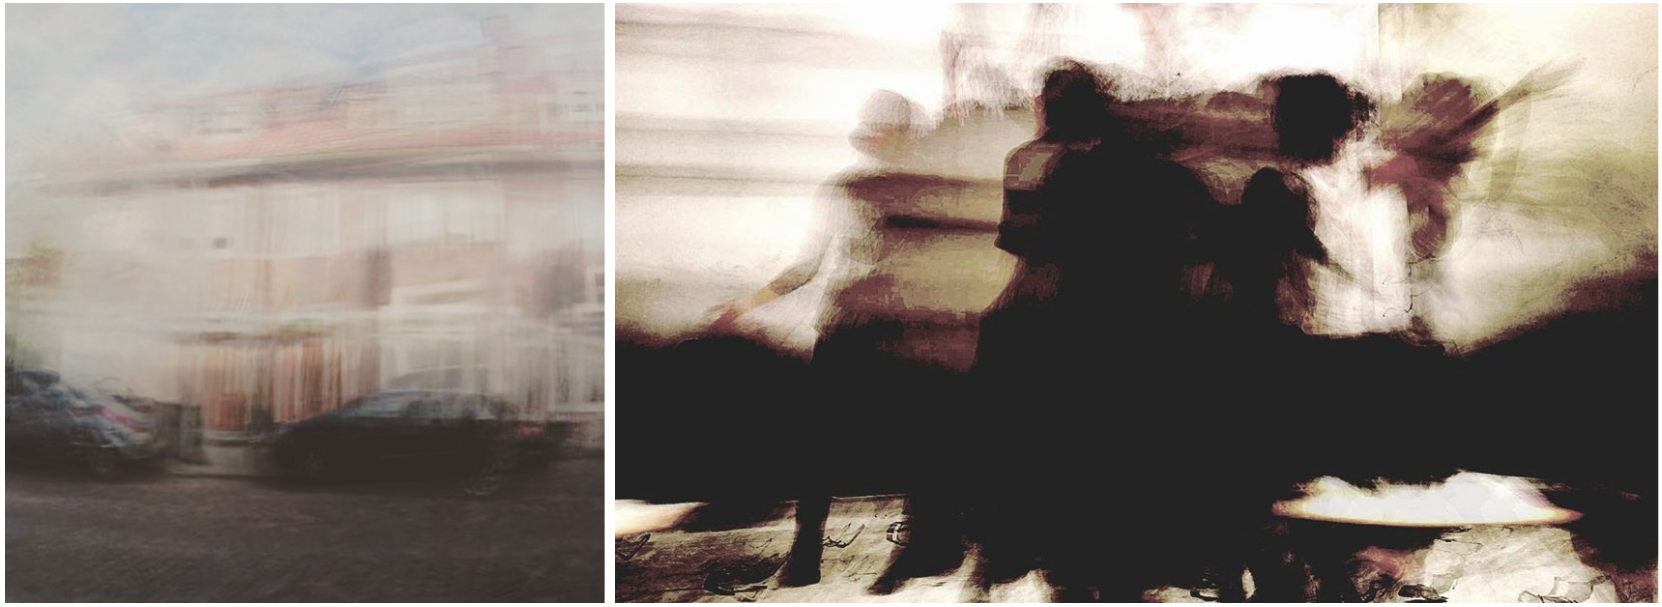
\includegraphics[width=0.8\linewidth]{assets/average.png} 
    \caption{\small \( u_{n+1} = u_{n} + \frac{x_{n+1} - u_{n}}{n+1} \) - \textit{Mauricio van der Maesen de Sombreff, video frames average}.}
    \label{fig:mv01}
\end{figure}

%% image
\begin{figure}
    \centering
    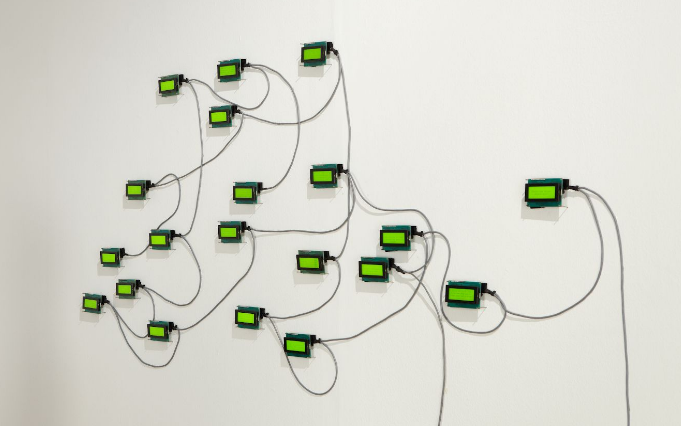
\includegraphics[width=0.8\linewidth]{assets/33_questions_per_minute_grifo.png} 
    \caption{\small Display version - \textit{Rafael Lozano-Hemmer, 33 questions per minute, https://www.lozano-hemmer.com}.}
    \label{fig:lozano}
\end{figure}

